\section{实验与分析}

\subsection*{目录}
\frame {
	\frametitle{目录}
    \tableofcontents[currentsection]
}

\subsection*{基于RDMA的对象传输性能测试}

\begin{frame}
	\frametitle{优化实现的传输性能}

	\begin{block}{总结}
		\begin{itemize}
			\item 32KB时切换协议:内存注册 vs. 内存拷贝
			\item 小对象:RDMA Send > RDMA Read $\approx $ Socket,1KB~15\%提升
			\item 大对象:RDMA Read > RDMA Send > Socket,4MB~7倍吞吐
		\end{itemize}
	\end{block}

	\vspace{-1em}
	\begin{columns}[t]
		\column{0.5\textwidth}
		\begin{figure}
			\centering
			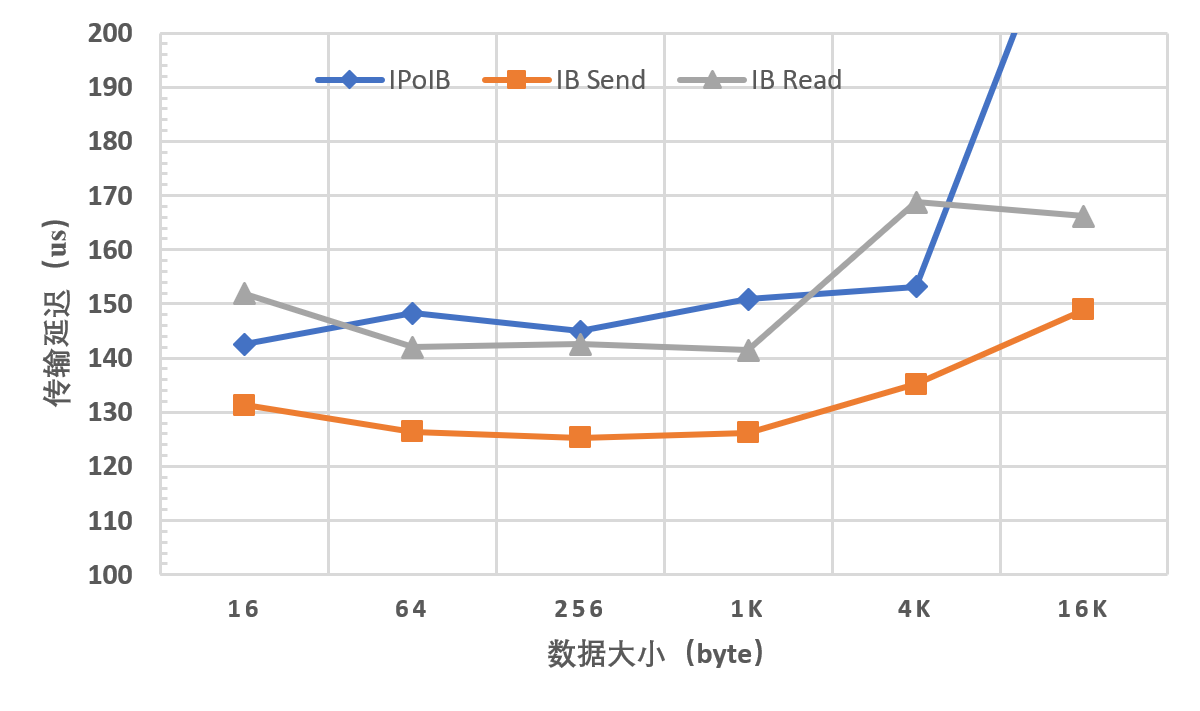
\includegraphics[width=\textwidth]{image/chap04/small.png}
			\caption{小对象传输性能}
		\end{figure}
		
		\column{0.5\textwidth}
		\begin{figure}
			\centering
			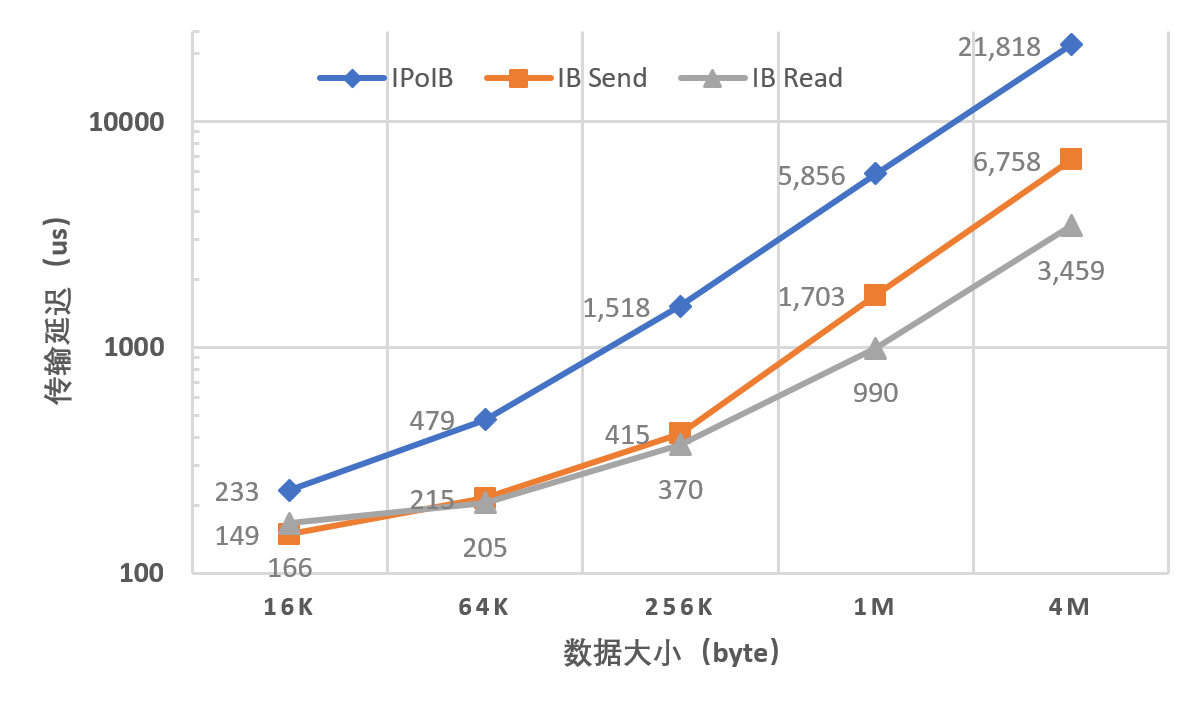
\includegraphics[width=\textwidth]{image/chap04/big.png}
			\caption{大对象传输性能}
		\end{figure}
	\end{columns}
\end{frame}

\begin{frame}
	\frametitle{Plasma(优化后) vs. Redis}

	\begin{block}{总结}
		\begin{itemize}
			\item 功能上:分布式存储(多副本)、分布式访问
			\item 性能上:常见大小对象的单机吞吐 \textbf{仍然} 更优
		\end{itemize}
	\end{block}

	\vspace{-1em}
	\begin{columns}[t]
		\column{0.5\textwidth}
		\begin{figure}
			\centering
			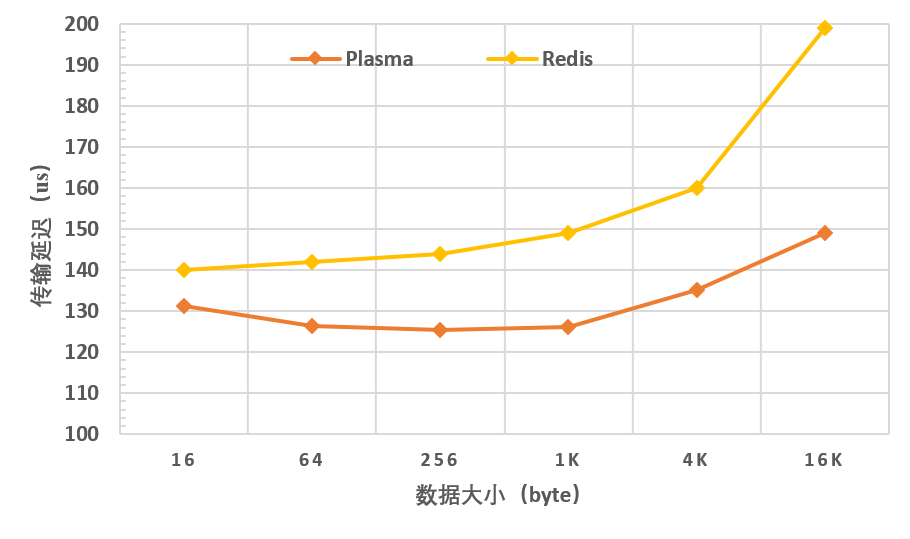
\includegraphics[width=\textwidth]{image/chap04/redis_small.png}
			\caption{小对象传输性能}
		\end{figure}
		
		\column{0.5\textwidth}
		\begin{figure}
			\centering
			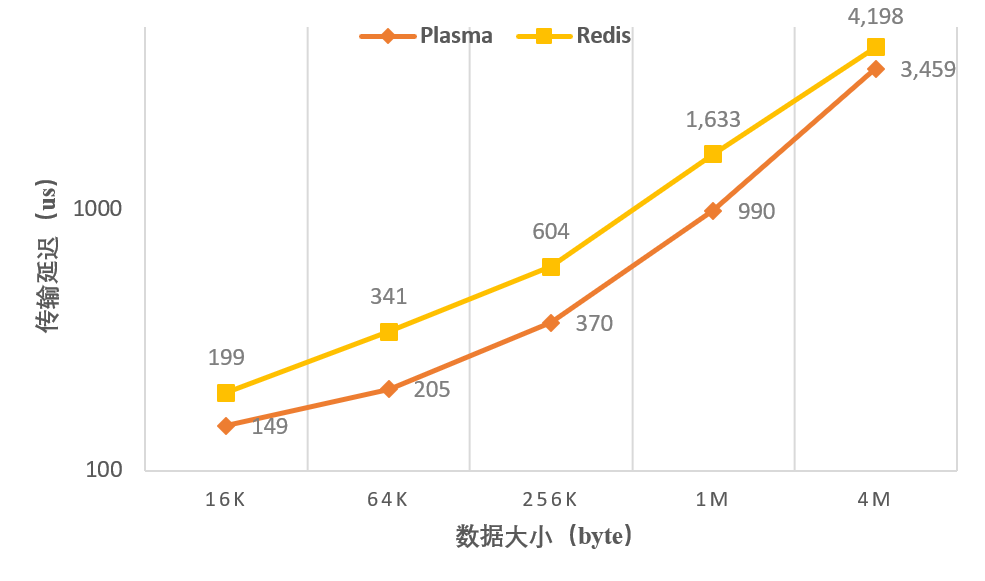
\includegraphics[width=\textwidth]{image/chap04/redis_big.png}
			\caption{大对象传输性能}
		\end{figure}
	\end{columns}
\end{frame}